\documentclass[border=6pt]{standalone}
\usepackage{tikz}
\usetikzlibrary{arrows.meta,positioning,shapes.geometric}
\begin{document}
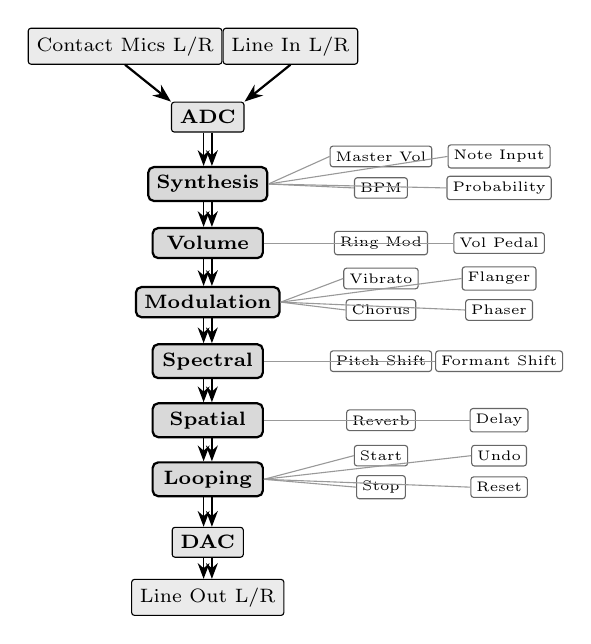
\begin{tikzpicture}

\node[rectangle, draw, fill=black!8, rounded corners=1pt, font=\scriptsize, inner sep=3pt] (cmic) at (-0.95, 1.6) {Contact Mics L/R};
\node[rectangle, draw, fill=black!8, rounded corners=1pt, font=\scriptsize, inner sep=3pt] (linein) at (1.15, 1.6) {Line In L/R};

\node[rectangle, draw, fill=black!10, rounded corners=1pt, font=\scriptsize\bfseries, inner sep=3pt] (adc) at (0.1, 0.7) {ADC};

\draw[-Stealth, thick] (cmic.south) -- (adc.north west);
\draw[-Stealth, thick] (linein.south) -- (adc.north east);

\node[rectangle, draw, thick, fill=black!15, rounded corners=2pt, font=\scriptsize\bfseries, inner sep=3pt, minimum width=1.4cm] (synth) at (0.1, -0.15) {Synthesis};
\node[rectangle, draw, thick, fill=black!15, rounded corners=2pt, font=\scriptsize\bfseries, inner sep=3pt, minimum width=1.4cm] (vol) at (0.1, -0.9) {Volume};
\node[rectangle, draw, thick, fill=black!15, rounded corners=2pt, font=\scriptsize\bfseries, inner sep=3pt, minimum width=1.4cm] (mod) at (0.1, -1.65) {Modulation};
\node[rectangle, draw, thick, fill=black!15, rounded corners=2pt, font=\scriptsize\bfseries, inner sep=3pt, minimum width=1.4cm] (spec) at (0.1, -2.4) {Spectral};
\node[rectangle, draw, thick, fill=black!15, rounded corners=2pt, font=\scriptsize\bfseries, inner sep=3pt, minimum width=1.4cm] (spat) at (0.1, -3.15) {Spatial};
\node[rectangle, draw, thick, fill=black!15, rounded corners=2pt, font=\scriptsize\bfseries, inner sep=3pt, minimum width=1.4cm] (loop) at (0.1, -3.9) {Looping};

\draw[-Stealth, semithick] ([xshift=-1.5pt]adc.south) -- ([xshift=-1.5pt]synth.north);
\draw[-Stealth, semithick] ([xshift=1.5pt]adc.south) -- ([xshift=1.5pt]synth.north);
\draw[-Stealth, semithick] ([xshift=-1.5pt]synth.south) -- ([xshift=-1.5pt]vol.north);
\draw[-Stealth, semithick] ([xshift=1.5pt]synth.south) -- ([xshift=1.5pt]vol.north);
\draw[-Stealth, semithick] ([xshift=-1.5pt]vol.south) -- ([xshift=-1.5pt]mod.north);
\draw[-Stealth, semithick] ([xshift=1.5pt]vol.south) -- ([xshift=1.5pt]mod.north);
\draw[-Stealth, semithick] ([xshift=-1.5pt]mod.south) -- ([xshift=-1.5pt]spec.north);
\draw[-Stealth, semithick] ([xshift=1.5pt]mod.south) -- ([xshift=1.5pt]spec.north);
\draw[-Stealth, semithick] ([xshift=-1.5pt]spec.south) -- ([xshift=-1.5pt]spat.north);
\draw[-Stealth, semithick] ([xshift=1.5pt]spec.south) -- ([xshift=1.5pt]spat.north);
\draw[-Stealth, semithick] ([xshift=-1.5pt]spat.south) -- ([xshift=-1.5pt]loop.north);
\draw[-Stealth, semithick] ([xshift=1.5pt]spat.south) -- ([xshift=1.5pt]loop.north);

\node[rectangle, draw, fill=black!10, rounded corners=1pt, font=\scriptsize\bfseries, inner sep=3pt] (dac) at (0.1, -4.7) {DAC};
\draw[-Stealth, semithick] ([xshift=-1.5pt]loop.south) -- ([xshift=-1.5pt]dac.north);
\draw[-Stealth, semithick] ([xshift=1.5pt]loop.south) -- ([xshift=1.5pt]dac.north);

\node[rectangle, draw, fill=black!8, rounded corners=1pt, font=\scriptsize, inner sep=3pt] (out) at (0.1, -5.4) {Line Out L/R};
\draw[-Stealth, semithick] ([xshift=-1.5pt]dac.south) -- ([xshift=-1.5pt]out.north);
\draw[-Stealth, semithick] ([xshift=1.5pt]dac.south) -- ([xshift=1.5pt]out.north);

\node[rectangle, draw=black!60, fill=white, rounded corners=1pt, font=\tiny, inner sep=2pt] at (2.3, 0.2) (s1) {Master Vol};
\node[rectangle, draw=black!60, fill=white, rounded corners=1pt, font=\tiny, inner sep=2pt] at (2.3, -0.2) (s2) {BPM};
\node[rectangle, draw=black!60, fill=white, rounded corners=1pt, font=\tiny, inner sep=2pt] at (3.8, 0.2) (s3) {Note Input};
\node[rectangle, draw=black!60, fill=white, rounded corners=1pt, font=\tiny, inner sep=2pt] at (3.8, -0.2) (s4) {Probability};
\draw[thin, black!40] (synth.east) -- (s1.west);
\draw[thin, black!40] (synth.east) -- (s2.west);
\draw[thin, black!40] (synth.east) -- (s3.west);
\draw[thin, black!40] (synth.east) -- (s4.west);

\node[rectangle, draw=black!60, fill=white, rounded corners=1pt, font=\tiny, inner sep=2pt] at (2.3, -0.9) (v1) {Ring Mod};
\node[rectangle, draw=black!60, fill=white, rounded corners=1pt, font=\tiny, inner sep=2pt] at (3.8, -0.9) (v2) {Vol Pedal};
\draw[thin, black!40] (vol.east) -- (v1.west);
\draw[thin, black!40] (vol.east) -- (v2.west);

\node[rectangle, draw=black!60, fill=white, rounded corners=1pt, font=\tiny, inner sep=2pt] at (2.3, -1.35) (m1) {Vibrato};
\node[rectangle, draw=black!60, fill=white, rounded corners=1pt, font=\tiny, inner sep=2pt] at (2.3, -1.75) (m2) {Chorus};
\node[rectangle, draw=black!60, fill=white, rounded corners=1pt, font=\tiny, inner sep=2pt] at (3.8, -1.35) (m3) {Flanger};
\node[rectangle, draw=black!60, fill=white, rounded corners=1pt, font=\tiny, inner sep=2pt] at (3.8, -1.75) (m4) {Phaser};
\draw[thin, black!40] (mod.east) -- (m1.west);
\draw[thin, black!40] (mod.east) -- (m2.west);
\draw[thin, black!40] (mod.east) -- (m3.west);
\draw[thin, black!40] (mod.east) -- (m4.west);

\node[rectangle, draw=black!60, fill=white, rounded corners=1pt, font=\tiny, inner sep=2pt] at (2.3, -2.4) (sp1) {Pitch Shift};
\node[rectangle, draw=black!60, fill=white, rounded corners=1pt, font=\tiny, inner sep=2pt] at (3.8, -2.4) (sp2) {Formant Shift};
\draw[thin, black!40] (spec.east) -- (sp1.west);
\draw[thin, black!40] (spec.east) -- (sp2.west);

\node[rectangle, draw=black!60, fill=white, rounded corners=1pt, font=\tiny, inner sep=2pt] at (2.3, -3.15) (st1) {Reverb};
\node[rectangle, draw=black!60, fill=white, rounded corners=1pt, font=\tiny, inner sep=2pt] at (3.8, -3.15) (st2) {Delay};
\draw[thin, black!40] (spat.east) -- (st1.west);
\draw[thin, black!40] (spat.east) -- (st2.west);

\node[rectangle, draw=black!60, fill=white, rounded corners=1pt, font=\tiny, inner sep=2pt] at (2.3, -3.6) (l1) {Start};
\node[rectangle, draw=black!60, fill=white, rounded corners=1pt, font=\tiny, inner sep=2pt] at (2.3, -4.0) (l2) {Stop};
\node[rectangle, draw=black!60, fill=white, rounded corners=1pt, font=\tiny, inner sep=2pt] at (3.8, -3.6) (l3) {Undo};
\node[rectangle, draw=black!60, fill=white, rounded corners=1pt, font=\tiny, inner sep=2pt] at (3.8, -4.0) (l4) {Reset};
\draw[thin, black!40] (loop.east) -- (l1.west);
\draw[thin, black!40] (loop.east) -- (l2.west);
\draw[thin, black!40] (loop.east) -- (l3.west);
\draw[thin, black!40] (loop.east) -- (l4.west);

\end{tikzpicture}
\end{document}
